\section{Necessary Data}
In order to create a suitable database schema, the first step is to figure out what should be in the database.
This analysis focuses on the structure of the institutions involved in the \ac{giraf} project. 

An institution can have several departments. Each department has a number of employees, hereafter referred to as
\emph{guardians}, assigned to it as well as some children that attend the department. Each department has one or
more administrators, an administrator is a guardian with some extra privileges and authority. Each guardian is
responsible for a few specific children, but is of course not limited to only taking care of the ones he or she
is responsible for. This is however something that they handle internally. As \autoref{fig:data_overview}
illustrates, each department has a number of guardians and children and one of the guardians acts as an
administrator for that department. Children are assigned to one specific department. Generally each department
has its own administrators, but in some cases a single administrator handles several departments.

\begin{figure}[hptb]
	\begin{center}
	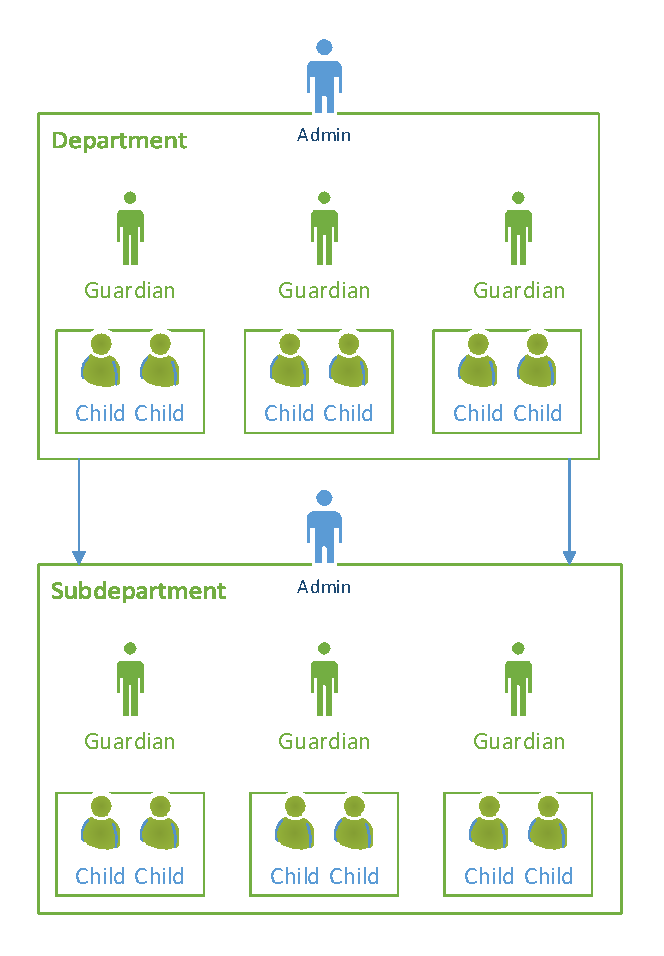
\includegraphics[width=0.8\textwidth]{img/data_overview.pdf}
	\caption{Overview of the people involved and department structure}
	\label{fig:data_overview}
	\end{center}
\end{figure} 

The children have needs and demands that can vary greatly from one child to another. But common for all of the
children is that they each have their own set of pictograms. The children generally have a resistance to change
e.g. the taxi that drives them to the institution and picks them up again has to have a specific colour. This
tendency can also occur with regard to preferences as some children insist on their pictograms being black and
white with stick figures and other prefer coloured images. 

When these things are applied to what could be used in the database schema, there is a need to be able to
represent \emph{departments} with optional \emph{subdepartments}. There needs to be a representation of
\emph{guardians} and \emph{children}. The system should also be able to give guardians \emph{administrator}
rights to departments. The \emph{pictograms} need to be included and it might be a good idea to be able to
categorize the pictograms e.g. cereal and milk under breakfast items.